\chapter{Segunda ley de la termodinámica}

\section{Procesos reversibles e irreversibles}

\subsection*{Procesos reversibles e irreversibles}

Otro aspecto importante es cómo evolucionan los sistemas entre estados termodinámicos. Joule fue
el primero en notar que, para un sistema aislado encerrado por paredes adiabáticas, cualesquiera
dos estados de equilibrio (por ejemplo $A$ y $B$) con el mismo número de moles $N_1,N_2,\dots,N_K$
pueden ser unidos por un proceso mecánico dado.

Joule descubrió que, para dos estados determinados $A$ y $B$, es posible encontrar procesos
mecánicos tales que
\begin{align*}
  A&\to B\quad\text{(llevar al sistema de $A$ a $B$)}\\
  \text{o}\quad B&\to A\quad\text{(llevar al sistema de $B$ a $A$)}
\end{align*}
pero \textbf{no ambos a la vez}; es decir, existe un proceso que lleva de $A$ a $B$ o de $B$ a
$A$, pero no ambos (Joule lo hizo para sistemas adiabáticos).

Esta asimetría entre dos estados se asocia con el concepto de \textbf{irreversibilidad}. Esto es
algo que siempre se ha observado en los sistemas termodinámicos, pero no hay ninguna razón de
primeros principios que justifique este hecho.

Sin embargo, podemos decir que, para un sistema aislado, su estado termodinámico especificado por
sus variables macroscópicas ($U,V,N$, entre otras) evolucionará \textbf{irreversiblemente} hacia
estados invariantes en el tiempo, en los cuales no ocurren más cambios físicos o químicos. Estos
estados son llamados \textbf{estados de equilibrio termodinámico}. La evolución de un sistema
hacia un estado de equilibrio ocurre debido a un \emph{proceso irreversible}, los cuales ocurren
solo en un sentido, pero no en reverso. Por ejemplo:
\begin{itemize}[itemsep=0pt]
  \item hielo derritiéndose;
  \item café mezclado con leche.
\end{itemize}
Más adelante discutiremos esto con más detalle.

\subsection*{La segunda ley de la termodinámica}

\begin{ley}[Segunda ley de la termodinámica]
  En un sistema cerrado la entropía tiende a aumentar con el tiempo. Asimismo (esto lo veremos
  después), el calor no puede fluir espontáneamente de un sistema con temperatura $T^{(1)}$ a otro
  con temperatura $T^{(2)}$ si $T^{(1)}<T^{(2)}$.
\end{ley}
% NOTA: el manuscrito escribe "si T^{(1)} > T^{(2)}"; se corrigió a "<" (el calor no fluye espontáneamente del más frío al más caliente). Verificar.

Diferencialmente se puede escribir la segunda ley en términos del tipo de proceso:
\begin{enumerate}[label=\arabic*.,itemsep=2pt]
  \item Para procesos reversibles, $\dd S=\dfrac{\dbar Q_{\mathrm{rev}}}{T}$.
  \item Para procesos irreversibles, $\dd S>\dfrac{\dbar Q}{T}$.
\end{enumerate}
En general, $\dd S\geq\dfrac{\delta Q}{T}$. Con esto tenemos las bases del marco teórico completo de
la termodinámica.

\subsection*{Procesos cuasiestáticos y reversibles}

Para describir y caracterizar estados termodinámicos y, posteriormente, describir posibles
procesos, suele ser útil definir un \textbf{espacio de configuración termodinámico}. El espacio de
configuración termodinámico para sistemas simples es un espacio abstracto definido por ejes
coordenados que corresponden a la entropía $S$ y a los parámetros extensivos $U,V,N_1,\dots,N_r$
del sistema.

La relación fundamental $S=S(U,V,N_1,\dots,N_r)$ define una hipersuperficie en el espacio de
configuración termodinámico.
\begin{figure}[H]
  \centering
  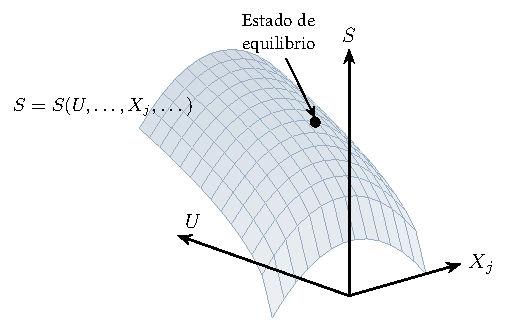
\includegraphics{figuras/sup-equilibrio.pdf}
\end{figure}
Esta hipersuperficie debe cumplir con los requerimientos usuales de que $U$ sea una función
univaluada de $S,\dots,X_j,\dots$ y $\pdvc{S}{U}{\dots,X_j,\dots}\equiv1/T$ sea positiva. Por definición,
cada punto en esta hipersuperficie representa un estado de equilibrio (para representar estados de
no equilibrio se necesita un espacio de mucho mayor dimensión).

Para sistemas compuestos (mezclas), estos pueden ser representados por una hipersuperficie en un
espacio de configuración termodinámico con ejes coordenados correspondientes a los parámetros
extensivos de todos los subsistemas.

Consideremos ahora el siguiente diagrama, donde una curva arbitraria parte desde un estado inicial
$A$ hasta un estado final $I$.
\begin{figure}[H]
  \centering
  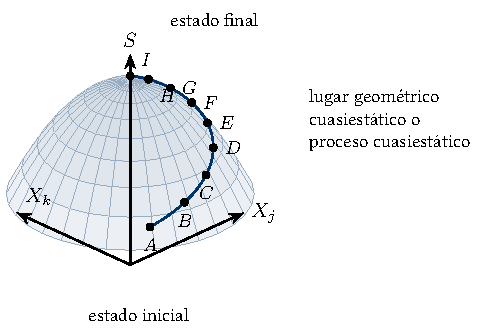
\includegraphics{figuras/sup-cuasiestatico.pdf}
\end{figure}
Tal curva es llamada \textbf{lugar geométrico cuasiestático} o \textbf{proceso cuasiestático}. Por lo
tanto, un proceso cuasiestático se define en términos de una \emph{sucesión densa de estados de
equilibrio}.

Por lo tanto, un proceso cuasiestático es un concepto idealizado, muy distinto de los procesos
reales, para los que siempre habrá estados fuera del equilibrio intermedios, los cuales no se pueden
representar en el espacio configuracional termodinámico. Asimismo, un proceso cuasiestático nunca
involucra tasas de cambio, velocidades o el tiempo.
\begin{itemize}[itemsep=0pt]
  \item \textbf{Proceso cuasiestático:} sucesión ordenada de estados de equilibrio.
  \item \textbf{Proceso real:} sucesión temporal de estados de equilibrio y de no equilibrio.
\end{itemize}

Aunque ningún proceso real es idéntico a un proceso cuasiestático, es posible llevar a un sistema
real a través de una sucesión de estados que coincidan con cualquier número de puntos deseados con
un dado lugar geométrico cuasiestático.

Por ejemplo, consideremos un sistema originalmente en el estado $A$ y el proceso cuasiestático que
pasa por el lugar geométrico de los puntos $A,B,C,\dots,H$; se remueven las restricciones que
permiten al sistema ir del estado $A$ al estado $B$, pero sin ir más allá. En este caso, el sistema
``desaparece'' del punto $A$ y ``aparece'' en el punto $B$, ya que pasó a través de estados fuera del
equilibrio. Si se relajan aún más las condiciones y se permite al sistema evolucionar al estado $C$,
el sistema desaparece de $B$ y aparece en $C$, y así con cada uno de los puntos del proceso
cuasiestático, con lo que se construye un proceso real como una aproximación a un proceso
cuasiestático. Al espaciar los puntos $A,B,\dots$ arbitrariamente tan cerca como se desee, se puede
aproximar al lugar geométrico del proceso cuasiestático tanto como se desee.

Para continuar, no olvidemos que la identificación de $-P\,\dd V$ con el trabajo mecánico y de
$T\,\dd S$ con el flujo de calor solo es válida para procesos cuasiestáticos.

Consideremos un sistema cerrado que es llevado a través de una secuencia de estados $A,B,\dots,H$
aproximándose a un lugar geométrico cuasiestático. El sistema es inducido para ir desde $A$ hasta $B$
al remover alguna restricción interna; el sistema pasará al estado $B$ si y solo si dicho estado
tiene máxima entropía de entre todos los nuevos estados accesibles. En particular,
\begin{equation*}
  S_B>S_A,\qquad A\to B\quad\text{pero}\quad B\not\to A.
\end{equation*}
Por lo cual, el proceso físico que une a los estados $A$ y $B$ es \emph{unidireccional}: desde el
estado $A$ de menor entropía al estado $B$ de mayor entropía, pero no a la inversa. Tal proceso es
llamado \textbf{irreversible}.

Por lo tanto, un lugar geométrico cuasiestático (trayectoria en el espacio configuracional
termodinámico) puede ser aproximado a un proceso real en un sistema cerrado si y solo si la entropía
es monótonamente no decreciente a lo largo de la trayectoria cuasiestática.

El caso límite en el que un proceso cuasiestático genere un incremento de entropía tan pequeño que
es despreciable es llamado \textbf{proceso reversible}. Tal proceso corresponde a una trayectoria
paralela al plano $X_k$--$X_j$ de entropía constante, y puede ser recorrido en cualquier dirección.
\begin{figure}[H]
  \centering
  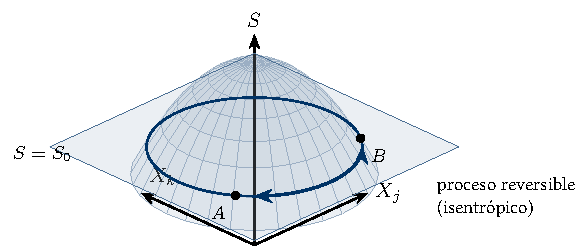
\includegraphics{figuras/sup-reversible.pdf}
\end{figure}

\section{Máquinas térmicas: ciclos de Carnot y otros}

\begin{observacion}[Temas omitidos]
  El manuscrito indica que se omiten los siguientes temas: tiempos de relajación e irreversibilidad;
  flujo de calor (sistemas acoplados y reversión de procesos); el teorema del máximo trabajo;
  coeficientes de rendimiento para motores, refrigeradores y bombas de calor; ciclo de Carnot;
  medibilidad de la temperatura y la entropía; otros criterios de rendimiento de motores (salida de
  potencia y motores endorreversibles); otros procesos cíclicos.
  % NOTA: en el manuscrito la penúltima viñeta dice "...salida de potencia y mot. ando reversibles"; se interpretó como "motores endorreversibles". Verificar.
\end{observacion}

